\documentclass[]{article}
\usepackage[utf8]{inputenc}
\usepackage{multicol}
\usepackage{amsmath}
\usepackage{amsthm}
\usepackage{amssymb}
\usepackage{bm}
\usepackage{physics}
\usepackage{graphicx}
\usepackage{float}
%\usepackage[round]{natbib}
%\bibliographystyle{unsrtnat}

% this just sets up the page size and margins
\setlength{\topmargin}{0pt}
\setlength{\oddsidemargin}{0pt}
\setlength{\evensidemargin}{0pt}
\setlength{\textwidth}{6.5in}
\setlength{\textheight}{8.5in}
\setlength{\headheight}{0pt}

% create some short cut commands
\newcommand{\bx}{\boldsymbol{x}}
\newcommand{\by}{\boldsymbol{y}}
\newcommand{\bu}{\boldsymbol{u}}


% this is a bunch of stuff that allows python style code snippits
% Default fixed font does not support bold face
\DeclareFixedFont{\ttb}{T1}{txtt}{bx}{n}{10} % for bold
\DeclareFixedFont{\ttm}{T1}{txtt}{m}{n}{10}  % for normal
% Custom colors
\usepackage{color}
\definecolor{deepblue}{rgb}{0,0,0.5}
\definecolor{deepred}{rgb}{0.6,0,0}
\definecolor{deepgreen}{rgb}{0,0.5,0}

\usepackage{listings}

% Python style for highlighting
\newcommand\pythonstyle{\lstset{
		language=Python,
		basicstyle=\ttm,
		morekeywords={self},              % Add keywords here
		keywordstyle=\ttb\color{deepblue},
		emph={MyClass,__init__},          % Custom highlighting
		emphstyle=\ttb\color{deepred},    % Custom highlighting style
		stringstyle=\color{deepgreen},
		frame=tb,                         % Any extra options here
		showstringspaces=false,
		tabsize=4
}}

% Python environment
\lstnewenvironment{python}[1][]
{
	\pythonstyle
	\lstset{#1}
}
{}

% Python for inline
\newcommand\pythoninline[1]{{\pythonstyle\lstinline!#1!}}

\title{Balancing Robot}
\author{Izzy Mones and Heidi Dixon}
%\date{}

\begin{document}
	\maketitle


 
\section*{Robot Design}
Should have list of all the components. Maybe a picture. Do we need to show circuit stuff?

\subsection*{Measuring the Robot State}
The position $x$ and velocity $\dot{x}$ along the $x$ axis are computed from the motor encoders. The encoders return a number of counts which is positive in the clockwise direction and negative in the counter clockwise direction. Using the number of counts per wheel rotation and the circumference of the wheel we can compute the distance in the $x$ direction. The instantaneous velocity can be estimated by computing the change in position over a very small time window times the length of the window. The angle $\theta$ is computed from the accelerometer and angular velocity $\dot{\theta}$ is given by the gyroscope.

\section*{Model}
Need a drawing of model.

Do we want a derive the equations?

We modeled our balancing robot as a pendulum cart system.The wheels and motors are considered to be the cart.  All other parts of the robot pivot around the axis created by the wheels and are considered part of the pendulum.   Our system is described by the system of differential equations

\begin{eqnarray}
	\dot{x} & = & \dot{x} \label{dfx} \\ 
	\ddot{x}          & = & \frac{-mg \cos(\theta)\sin(\theta) + mL{\dot{\theta}}^2 \sin(\theta)-\delta \dot{x}+u }{M+m\sin^2\theta}  \label{dfv} \\
	\dot{\theta}  &= & \dot{\theta} \label{dftheta} \\	
	\ddot{\theta}  &= & \frac{(m+M)g\sin(\theta)-\cos(\theta)(mL{\dot{\theta}}^2\sin(\theta)-\delta \dot{x})-\cos(\theta)u}{L(M+m\sin^2\theta)} \label{dfomega}
\end{eqnarray}
where $x$ is the cart position, $\dot{x}$ is the cart velocity, $\theta$ is the pendulum angle, $\dot{\theta}$ is the angular velocity, $m$ is the pendulum mass, $M$ is the cart mass, $L$ is the distance from the pivot point to the center of mass of the pendulum, $g$ is the gravitational acceleration, $\delta$ is a friction damping on the cart, and $u$ is the control force applied to the cart. This forms a set of differential equations 
\begin{equation}
	\frac{d}{dt} \bx = f(\bx, \bu) \label{dfdx}
\end{equation}
where $\bx$ is the state vector $\bx = [x, \dot{x}, \theta, \dot{\theta}]$ and $\bu$ is the input vector $\bu=[u]$.

\subsection*{Modeling Motors}
Talk about how we didn't model motor circuit. We assumed that torque is a linear function of duty cycle.  We tuned the coefficient experimentally.  This model is probably pretty good as long as are not near their max duty cycle. Why?

\subsection*{Linearization}
To build a control system for our model we will linearize the non-linear system of equations \eqref{dfx}, \eqref{dfv}, \eqref{dftheta}, and \eqref{dfomega} around a fixed point $(\bx_r, \bu_r)$  where $\bx_r$ is the position where the robot is vertical, unmoving and positioned at the origin and $\bu_r$ is the input with motor torque at zero.

The nonlinear system of differential equations \eqref{dfdx} can be represented as a Taylor series expansion around the point $(\bx_r, \bu_r)$.
\begin{equation}
	 f(\bx, \bu) = f(\bx_r, \bu_r) + \left.  \frac{\boldsymbol{df}}{\boldsymbol{dx}} \right|_{x_r}(\bx -\bx_r) 
	 + \left.  \frac{\boldsymbol{df}}{\boldsymbol{du}} \right|_{u_r}(\bu -\bu_r) 
	 + \left. \frac{\boldsymbol{d}^2\boldsymbol{f}}{\boldsymbol{dx}^2} \right|_{x_r}(\bx -\bx_r)^2
	 + \left. \frac{\boldsymbol{d}^2\boldsymbol{f}}{\boldsymbol{du}^2} \right|_{u_r}(\bu -\bu_r)^2 + \cdots
\end{equation}
Because $(\bx_r, \bu_r)$ is a fixed point, we know that $f(\bx_r, \bu_r) = 0$. Additionally, this approximation is only accurate in a small neighborhood around $(\bx_r, \bu_r)$.  In this neighborhood, we can assume that the values of both $(\bx -\bx_r)$ and $(\bu -\bu_r)$ are small, so higher order terms of this series will go to zero. So a fair estimate of our system is
\begin{equation}
	\frac{d}{dt} \bx \simeq \left.  \frac{\boldsymbol{df}}{\boldsymbol{dx}} \right|_{x_r}(\bx -\bx_r) 
	+  \left.  \frac{\boldsymbol{df}}{\boldsymbol{du}} \right|_{u_r}(\bu -\bu_r) 
\end{equation}
where $\left.  \frac{\boldsymbol{df}}{\boldsymbol{dx}} \right|_{x_r}$ is the Jacobian matrix for our system of equations $f(\bx, \bu)$ with respect to $\bx$ and $\left.  \frac{\boldsymbol{df}}{\boldsymbol{du}} \right|_{u_r}$ is the Jacobian matrix with respect to $\bu$. Both are then evaluated at the fixed point $(\bx_r, \bu_r)$.  Our partial differentials with respect to $\bx$ are

\begin{equation*}
	\pdv{f_1}{x}  = \pdv{f_1}{\theta} = \pdv{f_1}{\dot{\theta}} = 	\pdv{f_3}{x}  =	\pdv{f_3}{\dot{x}} = \pdv{f_3}{\theta} = 0 
\end{equation*}
\begin{equation*}
	 \pdv{f_1}{\dot{x}} = \pdv{f_3}{\dot{\theta}}  = 1
\end{equation*}


\begin{eqnarray*}
	\pdv{f_2}{x} = & 0 \\
	\pdv{f_2}{\dot{x}} =&  \frac{-\delta}{M + m \sin^2 \theta} \\
	\pdv{f_2}{\theta} =  & \frac{(M+ m \sin^2 \theta)(-mg(\cos^2 \theta - \sin^2 \theta)+mL\dot{\theta}^2 \cos \theta)-(-mg \cos(\theta)\sin(\theta) + mL{\dot{\theta}}^2 \sin(\theta)-\delta \dot{x}+u)(2m \sin \theta \cos \theta)}{(M + m \sin^2 \theta)^2} \\
	\pdv{f_2}{\dot{\theta}} = & \frac{mL\sin \theta}{M + m \sin^2 \theta} \cdot 2 \dot{\theta}
\end{eqnarray*}

\begin{eqnarray*}
	\pdv{f_4}{x} = & 0 \\
	\pdv{f_4}{\dot{x}} =&  \frac{\delta \cos \theta}{L(M + m \sin^2 \theta)} \\
	\pdv{f_4}{\theta} =  &  \frac{(L(M + m \sin^2 \theta))((M+m)g \cos \theta -mL\dot{\theta}^2(\cos^2 \theta - \sin^2 \theta) -\delta \dot{x} \sin \theta + u \sin \theta)}{L^2(M + m \sin^2 \theta)^2} \\
	& - \frac{((m+M)g\sin(\theta)-\cos(\theta)(mL{\dot{\theta}}^2\sin(\theta)-\delta \dot{x})-\cos(\theta)u)(2mL \sin \theta \cos \theta)}{L^2(M + m \sin^2 \theta)^2} \\
	\pdv{f_4}{\dot{\theta}} = & -\frac{2\dot{\theta}mL \cos \theta \sin \theta}{L(M + m \sin^2 \theta)}
\end{eqnarray*}
The Jacobian matrix for our system of equations evaluated at $\bx_r = [0\; 0\; \pi \; 0]$ and $\bu_r = [0]$ gives the matrix
\begin{equation}
		A = 
	\begin{bmatrix}
		0 & 1              & 0                          & 0 \\
		0 & -\frac{\delta}{M}      & -\frac{mg}{M}                 & 0 \\
		0 & 0              & 0                          & 1 \\
		0 & -\frac{\delta}{ML} & -\frac{(m+M)g}{ML} & 0
	\end{bmatrix} \label{A}
\end{equation}
Our partial differentials with respect to $\bu$ are
\begin{eqnarray*}
	\pdv{f_1}{u} = & 0 \\
	\pdv{f_2}{u} = & \frac{1}{M + m \sin^2 \theta}\\
	\pdv{f_3}{u} =  & 0 \\
	\pdv{f_4}{u} = & -\frac{\cos \theta}{L(M + m \sin^2 \theta)}
\end{eqnarray*}
Evaluating these equations at $\bx_r = [0\; 0\; \pi \; 0]$ and $\bu_r = [0]$ gives the matrix
\begin{equation}
	B = 
	\begin{bmatrix}
		0 \\
		\frac{1}{M}  \\
		0  \\
		\frac{1}{ML}   
	\end{bmatrix}
\end{equation}
Now we can approximate our system of equations \eqref{dfx}, \eqref{dfv}, \eqref{dftheta}, and \eqref{dfomega} with the linear system
\begin{equation}
	\frac{d}{dt} \bx = A(\bx - \bx_r) + B (\bu - \bu_r). \label{lin_mod}
\end{equation}
\subsection*{Two Variable Model}
We also built a two variable model for the balancing robot that has a state consisting of only the robot angle and angular velocity. This model works if you don't need to control the position of the robot. Working with this model was useful for testing purposes since it is a simpler system. It has the equations of motion
\begin{eqnarray*}
	\dot{\theta}  &= & \dot{\theta} \\	
	\ddot{\theta}  &= & \frac{(m+M)g\sin(\theta)-\cos(\theta)(mL{\dot{\theta}}^2\sin(\theta))-\cos(\theta)u}{L(M+m\sin^2\theta)} 
\end{eqnarray*}
and the linearized matrices
\begin{equation*}
		A = 
\begin{bmatrix}
	0                          & 1 \\
	-\frac{(m+M)g}{ML} & 0
\end{bmatrix}
\end{equation*}
\begin{equation*}
	B = 
	\begin{bmatrix}
		0  \\
		\frac{1}{ML}   
	\end{bmatrix}
\end{equation*}

\section*{Algorithms}
\subsection*{Linear Quadratic Regulator}
A Linear Quadratic Regulator (LQR) is a closed loop feedback system that uses a linearized model of the system based on differential equations to compute the optimal control parameters to stabilize the system around a fixed point. Additionally, LQR control allows some level of optimization over performance requirements, allowing tradeoffs between reducing the power consumption of our motors and the stability of the system. Our LQR algorithm and accompanying simulations were coded using Python's Control Systems library \pythoninline{control} and the numerical and scientific computing library \pythoninline{numpy}.

We need our linear system \eqref{lin_mod} to be {\bf controllable}. A system is controllable if the column space of the controllability matrix 
\begin{equation}
	\mathcal{C} = 
	\begin{bmatrix}
		B & AB & A^2B & \cdots & A^{n-1}B
	\end{bmatrix}
\end{equation}
has $n$ linearly independent columns, where $n$ is the number of variables in our state. At a high-level, controllability means that our control $B\bu$ has the ability to affect all of our state variables in $\bx$.  This is easily tested in Python with the line
\vspace{\baselineskip}
\begin{python}
	print(np.linalg.matrix_rank(ctrb(A, B)))
\end{python}
\vspace{\baselineskip}
For our system, the controllability matrix has rank $4$ confirming that our system is controllable.

LQR works by finding a  matrix $K$ that we can use to compute our control input $\bu$ from the current state $\bx$
\begin{equation}
	\bu = -K(\bx - \bx_r). \label{u}
\end{equation}
We know that the bahaviour of our system can be approximated with our linearized model  \eqref{lin_mod}. If we substitute \eqref{u} into  \eqref{lin_mod} we get
\begin{equation*}
 A(\bx - \bx_r) + B(-K(\bx - \bx_r)) = 	(A - BK)(\bx - \bx_r) 
\end{equation*}
In a controllable system we can select a matrix $K$ to make the real parts of all eigenvalues of  $A - BK$ have negative values.  This creates a stable system.  

To select our matrix $K$, we define two diagonal matrices $Q$ and $R$. $Q$ contains weights for the cost of deviating from the goal state and $R$ weights the cost of our control inputs. We use the Python \pythoninline{control.matlab.lqr} command to pick a $K$ that minimizes a cost function built from $Q$ and $R$. If the weight in $R$ is low relative to the weights in $Q$, our choice of $K$ will favor sticking close to our goal state with minimal limits on the size of motor torque. This can cause the robot to respond agressively to changes in state and make it overly sensitive to noise.  Typically, an LQR implementation will require some tuning of the weights in $Q$ and $R$ to meet the requirements of the system.
\vspace{\baselineskip}
\begin{python}
	from control.matlab import lqr
	
	# equations of motion linearized about vertical pendulum position
	A = np.array([[0, 1, 0, 0],\
				[0, -d/M, -m*g/M, 0],\
				[0, 0, 0, 1],\
				[0, -d/(M*L), -(m+M)*g/(M*L), 0]])
	
	# linearization of control matrix
	B = np.array([0,1/M,0,1/(M*L)]).reshape((4,1))
	
	Q = np.array([[1, 0, 0, 0],\
				[0, 0.01, 0, 0],\
				[0, 0, 10, 0],\
				[0, 0, 0, 0.1]])
	R = 1
	K = lqr(A,B,Q,R)[0]
\end{python}

A properly tuned $K$ matrix can be used in the control loop to compute the motor torque required to respond to the current state.  This value is then used to power the motors.
\vspace{\baselineskip}
\begin{python}
	def loop_iteration():
		theta, theta_dot = imu_sensor.angle_data()
		x, x_dot = motors.position_data()
		current_state = np.array([x, x_dot, theta, theta_dot])
		u = -K@(current_state - x_r)
		motors.run(u * duty_coeff)
\end{python}

\subsection*{Linear Quadratic Gaussian}
Need a discussion here of why we switched to LQG. What were the drawbacks of LQR approach? Like we don't have a way to measure velocity directly, we can only estimate it from the change in position over a short time window.  It's better to let the model estimate it because the model knows more about the behaviour of the system.

A linear quadratic gaussian algortihm (LQG) is an extension of the LQR method with two advantages.  It doesn't require sensor readings for all of the state variables and it can filter out noisy sensor data. Instead of reading the current state directly from the sensors, the algorithm estimates the current state using readings from the sensors together with predictions about the state from the linear model. State variables without sensors readings are estimated entirely. 

Because we may only have measurements for some of our state values we will need a measurement model described by a matrix.
\begin{equation}
	C = 
	\begin{bmatrix}
		1 & 0 & 0 & 0 \\
		0 & 0 & 1 & 0 \\
		0 & 0 & 0 & 1
	\end{bmatrix} \label{C}
\end{equation}	
The matrix $C$ for our implentation indicates that state variables $x$, $\theta$ and $\dot{\theta}$ will be measured.  We now need to show that our system is {\bf observable}. Observability is a dual concept to controllability. At a high-level, a system is observable if the measured variables have the ability to predict all the state variables in $\bx$.  For example, the measurement model $C = [1, 0, 0, 0]$ that measures only the position $x$ together with our $A$ matrix \eqref{A} is observable but the measurement model $C = [0, 0, 1, 0]$ that measures only the angle $\theta$ is not.  The angle $\theta$ can be constructed from the position $x$, but the reverse is not true. The $x$ position cannot be constructed fully from the angle $\theta$.  I need to study this a little more until I understand it.

A system is observable with measurement model $C$ if the rows of the observability matrix
\begin{equation}
	\mathcal{O} = 
	\begin{bmatrix}
		C \\ CA \\ CA^2 \\ \vdots \\ CA^{n-1}
	\end{bmatrix}
\end{equation}
span all of $\mathbb{R}^n$. We used the control library command \pythoninline{control.matlab.obsv} to construct the observability matrix for our measurement model \eqref{C}.  Observability can be demonstrated by taking the transpose of the observability matrix and testing that it's columns are full rank.  

We derive the Kalman filter matrix $K_f$ using the   \pythoninline{lqr} function from python control library. Our cost matrices $Q$ and $R$ will now represent the cost of deviating from the state, or disturbances, relative to deviations from the sensors, or noise. On a high-level this tells the model how much to trust the predictions of the model and how much to trust the readings from the sensors.
\vspace{\baselineskip}
\begin{python}
	# C is our measurement model
	C = np.array([[1, 0, 0, 0], \
				[0, 0, 1, 0], \
				[0, 0, 0, 1]]) 

	# This is our state disturbance matrix
	Q = np.eye(4) 

	# This is our sensor noise matrix
	R = np.eye(3)

	# Generate our Kalman Filter
	Kf = lqr(A.transpose(), C.transpose(), Q, R)[0].transpose()
\end{python}
\vspace{\baselineskip}

To build the linear state space for our Kalman filter
\begin{equation}
	\frac{d}{dt} \bx  = A_{kf} (\bx - \bx_r) + B_{kf} (\bu - \bu_r)  \label{lin_mod_kf}
\end{equation}
we build the new matrices
\begin{eqnarray*}
	A_{kf} = A - K_fC \\
	B_{kf} = \begin{bmatrix} B & K_f \end{bmatrix}
\end{eqnarray*}
Our input vector $\bu = [u, x_s, \theta_s, \dot{\theta}_s]$ is our motor torque $u$ and our  sensor readings, position $x_s$, angle $\theta_s$, and angular velocity $\dot{\theta}_s$
\vspace{\baselineskip}
\begin{python}
	def loop_iteration():
		# estimate the state
		dx = A_kf@(x - x_r) + B_kf@(u - u_r)
		x = x + dx*dt
	
		# read sensors and compute torque
		theta, theta_dot = imu_sensor.angle_data()
		x = motors.position_data()
		torque = -md.K@(x - x_r)  		
		u = np.array([torque, x, theta, theta_dot])
		motors.run(u[0] * duty_coeff)
\end{python}
\vspace{\baselineskip}
\subsection{Simulations with Python}
\begin{figure}[H]
	\centering
	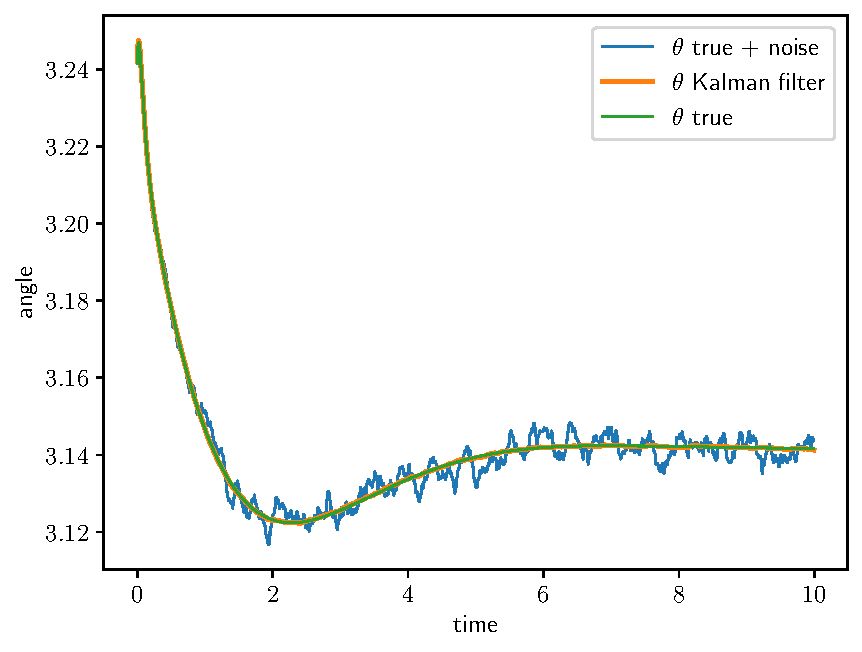
\includegraphics[width=0.8\linewidth]{KFangle.pdf}
	\caption{Simulation comparison of Kalman filter state estimation of angle with the true angle and noisy data.}
	\label{fig:kfangle}
\end{figure}

\begin{figure}[H]
	\centering
	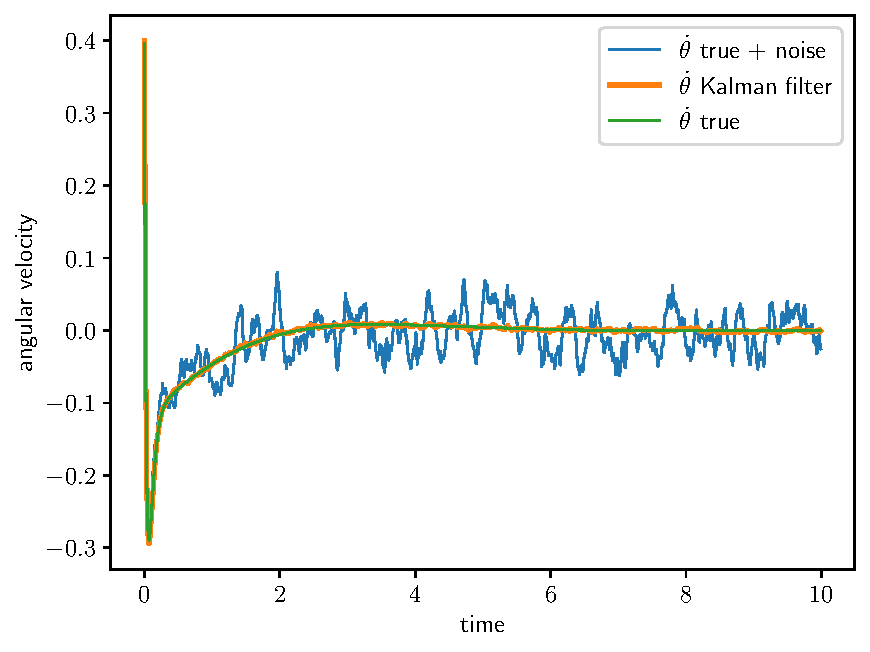
\includegraphics[width=0.8\linewidth]{KFangular_velocity.pdf}
	\caption{Simulation comparison of Kalman filter state estimation of angular velocity with the true angular velocity and noisy data.}
	\label{fig:kfangvel}
\end{figure}

\subsection*{Continuous vs. Discrete Models}
Linear systems can be model as continuous or discrete.  A continuous system \eqref{lin_mod} tells us how the system is changing.  The state is estimated by multiplying this change in state \pythoninline{dx} by a time delta \pythoninline{dt} and then adding that to the previous state.
\vspace{\baselineskip}
\begin{python}
	# estimate the state
	dx = A@(x - x_r) + B@(u - u_r)
	x = x + dx*dt
\end{python}
\vspace{\baselineskip}
A discrete system estimates the current state $\bx_{k+1}$ from the previous state $(\bx_k, \bu_k)$
\begin{equation}
	\bx_{k+1} = A_d \bx_k + B_d \bu_k
\end{equation}
where $\bx_{k+1} = \bx_k + \Delta t$,
\begin{equation*}
	A_d = e^{A \Delta t} 
\end{equation*}
\begin{equation*}
		B_d =  \int_0^{\Delta t} e^{A \Delta t}Bd\tau
\end{equation*}
and $e^{A \Delta t} $ is the matrix exponential.
Python's \pythoninline{control} library can create a discrete system from a continuous one. 
\vspace{\baselineskip}
\begin{python}
	# construct discrete system from a continuous system
	sys_c = ss(A, B, C, np.zeros_like(B))
	sys_d = c2d(sys_c, dt, 'zoh')
\end{python}
\vspace{\baselineskip}
Then the current state can be estimated from the previous state.
\vspace{\baselineskip}
\begin{python}
	x = sys_d.A@(x - x_r) + sys_d.B@(u - u_r) + x_r
\end{python}
We simulated both methods and found they produced very similar results.
\vspace{\baselineskip}
\begin{figure}[H]
	\centering
	\includegraphics[width=0.8\linewidth]{cont_vs_disc.pdf}
	\caption{Simulation comparing continuous and discrete methods for state estimation.}
	\label{fig:kfangvel}
\end{figure}
The discrete method was slightly faster at $4.1 \times 10^{-6}$ seconds per iteration with the continuous method taking $4.7 \times 10^{-6}$ seconds per iteration.
\section*{Experiments}

\section*{Conclusions}



\nocite{*}

\bibliographystyle{annotate}
\bibliography{references.bib}
\end{document}